\documentclass{article}
\usepackage{amsmath}
\usepackage{amssymb}
\usepackage{amsmath}
\usepackage{amssymb}
\usepackage{tikz}
\usetikzlibrary{automata, positioning, arrows}



\begin{document}
	
	Analyzing the concept of \textit{Moral Decision Making} in the context of predicate logic involves interpreting various linguistic elements within a logical framework. 
	
	\begin{itemize}
		\item \textbf{The Word "Decision"}: In predicate logic, "Decision" can be a constant or a variable. 
		\begin{itemize}
			\item As a constant (for a specific decision), it might be represented as \( d \).
			\item As a variable (representing any decision), it could be denoted as \( x \), where \( x \) is a decision.
		\end{itemize}
		
		\item \textbf{The Noun Phrase "Decision Making"}: "Decision Making" can be interpreted as a function in predicate logic. 
		\begin{itemize}
			\item The function \( \text{DecisionMaking}(x) \) represents the output or consequence of making decision \( x \).
		\end{itemize}
		
		\item \textbf{The Adjective "Moral" in "Moral Decision Making"}: "Moral" is a modifier and can be viewed as a predicate.
		\begin{itemize}
			\item The predicate \( \text{Moral}(\text{DecisionMaking}(x)) \) indicates that the decision-making process of \( x \) is of a moral nature.
		\end{itemize}
	\end{itemize}
	
	A typical formula connecting these elements might be:
	
	\[ \forall x (\text{Decision}(x) \rightarrow \text{Moral}(\text{DecisionMaking}(x))) \]
	
	This formula can be interpreted as: "For all \( x \), if \( x \) is a decision, then the decision-making process of \( x \) is moral." It employs a universal quantifier (\( \forall \)) to express a general statement about all decisions.
	
	In moral philosophy, these logical structures assist in defining and debating ethical theories and concepts, enabling a rigorous analysis of the nuances of moral decision-making.
	
	The concept of \textit{Moral Decision Making} can be analyzed using predicate logic, which provides a framework for understanding the linguistic and logical aspects of this philosophical concept.
	
	\begin{itemize}
		\item \textbf{The Word "Decision"}: In predicate logic, "Decision" can function as either a constant or a variable. 
		\begin{itemize}
			\item As a \textit{constant}, it represents a specific decision, typically denoted as \( d \).
			\item As a \textit{variable}, it symbolizes any decision, represented by \( x \), where \( x \) can be any decision.
		\end{itemize}
		
		\item \textbf{The Noun Phrase "Decision Making"}: This can be conceptualized as a function in predicate logic. 
		\begin{itemize}
			\item The function \( \text{DecisionMaking}(x) \) signifies the output or consequence that results from making decision \( x \).
		\end{itemize}
		
		\item \textbf{The Adjective "Moral" in "Moral Decision Making"}: Here, "Moral" functions as a predicate.
		\begin{itemize}
			\item The predicate \( \text{Moral}(\text{DecisionMaking}(x)) \) indicates that the decision-making process concerning \( x \) is characterized by moral considerations.
		\end{itemize}
	\end{itemize}
	
	A formula that captures the relationship between these elements is:
	
	\[ \forall x (\text{Decision}(x) \rightarrow \text{Moral}(\text{DecisionMaking}(x))) \]
	
	This formula is interpreted as: "For all \( x \), if \( x \) is a decision, then the decision-making process concerning \( x \) is moral." It employs a universal quantifier (\( \forall \)) to articulate a general statement about all decisions.
	
	In moral philosophy, applying predicate logic to concepts like moral decision-making aids in precisely defining and debating ethical theories and concepts. It allows for the structured and rigorous analysis of the subtleties involved in making moral decisions.
	
	The concept of \textit{Moral Decision Making} can be more accurately represented in predicate logic by considering that not all decisions are inherently moral, but rather, they become moral under certain conditions.
	
	Consider the revised approach:
	
	\begin{itemize}
		\item \textbf{Existential Quantification and Conditionality}: The formula should reflect that only some decisions fall under the category of moral decisions, contingent upon specific conditions being met.
	\end{itemize}
	
	A more realistic formula would be:
	
	\[ \exists x (C(x) \rightarrow (\text{Decision}(x) \land \text{Moral}(\text{DecisionMaking}(x)))) \]
	
	Here, \( C(x) \) represents the specific conditions under which a decision \( x \) can be considered moral. The formula is interpreted as: "There exists some decision \( x \) such that if the conditions \( C(x) \) are met, then \( x \) is a decision and the decision-making process concerning \( x \) is moral."
	
	This formula acknowledges that morality in decision-making is not a universal attribute of all decisions, but rather a characteristic of certain decisions under specific circumstances. Identifying and analyzing these conditions \( C(x) \) is a key aspect of ethical philosophy and moral reasoning.
	
	The concept of \textit{Moral Decision Making} can be more accurately represented in predicate logic by considering that not all decisions are inherently moral, but rather, they become moral under certain conditions.
	
	Consider the revised approach:
	
	\begin{itemize}
		\item \textbf{Existential Quantification and Conditionality}: The formula should reflect that only some decisions fall under the category of moral decisions, contingent upon specific conditions being met.
	\end{itemize}
	
	A more realistic formula would be:
	
	\[ \exists x (C(x) \rightarrow (\text{Decision}(x) \land \text{Moral}(\text{DecisionMaking}(x)))) \]
	
	Here, \( C(x) \) represents the specific conditions under which a decision \( x \) can be considered moral. The formula is interpreted as: "There exists some decision \( x \) such that if the conditions \( C(x) \) are met, then \( x \) is a decision and the decision-making process concerning \( x \) is moral."
	
	This formula acknowledges that morality in decision-making is not a universal attribute of all decisions, but rather a characteristic of certain decisions under specific circumstances. Identifying and analyzing these conditions \( C(x) \) is a key aspect of ethical philosophy and moral reasoning.
	
	
	Reexamining the concept of \textit{Moral Decision Making} in predicate logic, it is crucial to define and differentiate between the decision itself (\( D(x) \)) and the decision-making process (\( DM(x) \)).
	
	\begin{itemize}
		\item \( D(x) \): Represents the statement that 'x is a decision'. It is a predicate that is true if 'x' qualifies as a decision.
		\item \( DM(x) \): Signifies the process or outcome of making the decision 'x'. It is a function that maps a decision to its associated decision-making process.
	\end{itemize}
	
	A refined formula that takes these definitions into account would be:
	
	\[ \exists x (C(x) \rightarrow (D(x) \land \text{Moral}(DM(x)))) \]
	
	In this formula, \( C(x) \) represents the specific conditions under which a decision \( x \) is considered moral. The formula is interpreted as: "There exists some decision \( x \) such that if the conditions \( C(x) \) are met, then \( x \) is a decision (as per \( D(x) \)) and the decision-making process of \( x \) (as per \( DM(x) \)) is moral."
	
	This approach provides a clearer and more precise representation of moral decision-making, distinguishing between the decision itself and the process of making that decision, and linking morality to specific conditions.
	
	
	Incorporating deontic concepts and the practical nature of decisions, the analysis of \textit{Moral Decision Making} can be expanded:
	
	\begin{itemize}
		\item \( O(x) \): Represents that decision \( x \) is obligatory.
		\item \( P(x) \): Indicates that decision \( x \) is permissible.
		\item \( DM(x) \rightarrow A(x) \): Signifies that the decision-making process \( DM(x) \) leads to action \( A(x) \).
	\end{itemize}
	
	A more comprehensive formula might be:
	
	\[ \exists x (C(x) \rightarrow (D(x) \land (O(x) \lor P(x)) \land \text{Moral}(DM(x)) \rightarrow A(x))) \]
	
	This formula posits that there exists a decision \( x \) such that, under conditions \( C(x) \), \( x \) is a decision that is either obligatory or permissible, the decision-making process is moral, and this leads to a corresponding action.
	
	This approach highlights the complexity of moral decision-making, integrating the deontic aspects of obligation and permission, the practical outcome in terms of actions, and the psychological underpinnings of judgment and decision processes.
	
	\begin{itemize}
		\item States and Actions: Define states as different scenarios in the decision-making process. Actions are transitions (decisions or judgments) between states.
		\item Agents and Choices: Model agents as decision-makers, with actions based on logical conditions such as obligations, permissions, and moral evaluations.
		\item Transitions: Use \( C(x) \), \( D(x) \), \( O(x) \), \( P(x) \), and \( DM(x) \) to define transition rules. These dictate how agents move between states.
		\item Moral Evaluation: Integrate \( \text{Moral}(DM(x)) \) in transition rules to assess moral implications of actions.
		\item Action Outcomes: Represent outcomes of actions (\( A(x) \)) as resulting states in the AATS.
	\end{itemize}
	
	\subsection*{Programming Implementation}
	Implement the AATS in a programming language, translating logical relations and conditions into algorithms.
	
	\subsection*{Example of a Labelled Transition}
	Consider a scenario where an agent must decide whether to tell the truth or lie in a given situation.
	
	\begin{itemize}
		\item States: Truth-Telling State (S1), Lying State (S2).
		\item Actions: Tell Truth (a1), Lie (a2).
		\item Agents evaluate \( C(x) \), \( D(x) \), \( O(x) \), \( P(x) \), and \( DM(x) \) to choose an action.
	\end{itemize}
	
	\begin{center}
		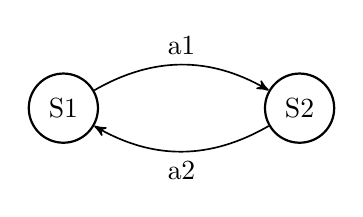
\begin{tikzpicture}[->, >=stealth', auto, semithick, node distance=3cm]
			\tikzstyle{every state}=[fill=white,draw=black,thick,text=black,scale=1]
			\node[state]    (S1)                     {S1};
			\node[state]    (S2)[right of=S1]   {S2};
			\path
			(S1) edge[bend left]  node{a1} (S2)
			(S2) edge[bend left]  node{a2} (S1);
		\end{tikzpicture}
	\end{center}
	
	In this graph, transitioning from S1 to S2 via action a1 represents the decision to tell the truth, considering the moral and practical implications of this action.
	
	Practical reason, as described in the Stanford Encyclopedia of Philosophy, is the general human capacity for resolving, through reflection, what one ought to do. It is practical in its subject matter, being concerned with action, and in its consequences or issue, as reflection about action directly moves people to act. Practical reason fundamentally differs from theoretical reason, as it is not concerned with the truth of propositions but with the desirability or value of actions.In practical reasoning, agents assess and weigh reasons for action, considering alternatives and the implications of each from a first-person perspective. This form of reasoning leads not to mere bodily movements but to intentional actions, which are grounded in our mental states and intentions. Thus, moral decision-making as an aspect of practical reason is indeed about the practical application of ethical principles in real-life situations, leading to actions based on moral judgments and considerations.
	
	Emotional reasoning plays a significant role in moral decision-making, serving as a bridge between practical reason and the realm of emotions. While practical reason focuses on the deliberation and resolution of what action to take, emotional reasoning adds a layer of subjective, affective evaluation to the decision-making process. This interplay can be understood in several ways:
	
	Moral Intuition: Emotions often serve as a source of moral intuition. They provide immediate, affective responses to moral situations, which can be crucial in the initial stages of practical reasoning.
	
	Motivation for Action: Emotions can motivate action, which is a key aspect of practical reason. Strong emotional responses can drive one to act in accordance with moral judgments.
	
	Evaluation of Consequences: Emotional reasoning is also involved in evaluating the consequences of actions, both for oneself and others, which is an essential part of ethical deliberation.
	
	Empathy and Moral Consideration: Emotional reasoning often involves empathy, which allows individuals to understand and respond to the emotions of others, an important factor in making moral decisions that affect others.
	
	Thus, emotional reasoning is intertwined with practical reason in moral decision-making, enriching the process with subjective, affective elements and ensuring that decisions are not just logically sound, but also emotionally resonant and empathetically considered.
	
	
	
	
	\section*{Moral Decision Making in Computing Science}
	
	In the interdisciplinary context of philosophy, psychology, and computing science, the concept of \textit{Moral Decision Making} is crucial in developing specifications for programs addressing moral dilemmas. Predicate logic offers a structured approach to conceptualize this idea.
	
	\subsection*{Logical Structure}
	\begin{itemize}
		\item \textbf{Decision Representation}: A decision can be a constant (\(d\)) or a variable (\(x\)), indicating a specific or generic decision.
		\item \textbf{Decision Making Function}: Represented as \( \text{DecisionMaking}(x) \), this function denotes the outcome of a decision \(x\).
		\item \textbf{Moral Predicate}: The predicate \( \text{Moral}(\text{DecisionMaking}(x)) \) suggests the moral aspect of decision-making for \(x\).
	\end{itemize}
	
	A key formula in this framework is:
	\begin{equation}
		\forall x (\text{Decision}(x) \rightarrow \text{Moral}(\text{DecisionMaking}(x)))
	\end{equation}
	signifying that all decisions \(x\) entail moral decision-making.
	
	However, recognizing the conditional nature of moral decisions, the formula is refined to:
	\begin{equation}
		\exists x (C(x) \rightarrow (\text{Decision}(x) \land \text{Moral}(\text{DecisionMaking}(x))))
	\end{equation}
	Here, \(C(x)\) are conditions making a decision \(x\) moral.
	
	\subsection*{Deontic and Action-Oriented Approach}
	Incorporating deontic logic and action-oriented perspectives, the formula evolves to:
	\begin{equation}
		\exists x (C(x) \rightarrow (D(x) \land (O(x) \lor P(x)) \land \text{Moral}(DM(x)) \rightarrow A(x)))
	\end{equation}
	This integrates obligation (\(O(x)\)), permission (\(P(x)\)), and actions (\(A(x)\)) into moral decision-making.
	
	\subsection*{Example with Graph}
	Consider an agent deciding between truth and lie:
	
	\begin{itemize}
		\item States: Truth-Telling State (S1), Lying State (S2).
		\item Actions: Tell Truth (a1), Lie (a2).
		\item Decision-making based on \(C(x)\), \(D(x)\), \(O(x)\), \(P(x)\), \(DM(x)\).
	\end{itemize}
	
	\begin{center}
		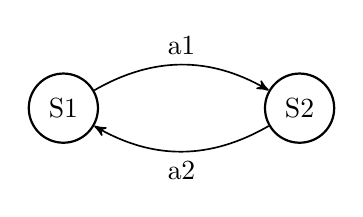
\begin{tikzpicture}[->, >=stealth', auto, semithick, node distance=3cm]
			\tikzstyle{every state}=[fill=white,draw=black,thick,text=black,scale=1]
			\node[state]    (S1)                     {S1};
			\node[state]    (S2)[right of=S1]   {S2};
			\path
			(S1) edge[bend left]  node{a1} (S2)
			(S2) edge[bend left]  node{a2} (S1);
		\end{tikzpicture}
	\end{center}
	
	Transitioning from S1 to S2 via action a1 represents choosing truth, factoring moral and practical implications.
	
	\subsection*{Conclusion}
	For computer scientists, this approach to \textit{Moral Decision Making} is instrumental in developing algorithms and programs for ethical problem-solving, blending logical reasoning with moral and deontic principles. This framework facilitates the translation of complex moral concepts into computable specifications, enabling machines to engage in ethical decision-making processes.
	
	
	
\end{document}
